\documentclass[a4paper]{report}

\usepackage{cite}
\usepackage[utf8]{inputenc}
\usepackage{makeidx}
\usepackage{a4wide}
\usepackage{setspace}
\usepackage{graphicx}
\usepackage{listing}
\usepackage{listings}
\usepackage{pslatex}
\usepackage[left=3cm,top=3cm,right=2cm,bottom=2cm]{geometry}

\makeindex
\begin{document}

\begin{titlepage}
\begin{center}
UNIVERSIDADE ESTADUAL DE MONTES CLAROS

Centro de Ciências Exatas e Tecnológicas

Departamento de Ciências da Computação

Curso de Sistemas de Informação
\\[2cm]
Herberth Giuliano Amaral Silva
\\[7cm]
\textbf {Uso de Uma Linguagem Específica de Domínio Baseada em XML Para Geração de Sistemas de Recuperação Estruturadas na Web na Linguagem Python}

\vfill
Montes Claros - MG

Dezembro - 2010



\end{center}
\end{titlepage}

%folha de rosto
\thispagestyle{empty}
\addtocounter{page}{-1}

\begin{center}
	Herberth Giuliano Amaral Silva
	\\[4cm]
	\textbf{Uso de Uma Linguagem Específica de Domínio Baseada em XML Para Geração de Sistemas de Recuperação Estruturadas na Web na Linguagem Python}
\end{center}
	\ \\[3cm]
	
\begin{flushright}
	\begin{small}
		\parbox{200pt}{Projeto orientado de conclusão de curso apresentado ao Curso de Sistemas de Informação,	da Universidade Estadual de Montes Claros como exigência para obtenção do grau de Bacharel	em Sistemas de Informação.}

		\parbox{200pt}{Orientador: Prof.Renato Dourado Maia.}
		
	\end{small}
\end{flushright}

\begin{center}	
	\vfill
	Montes Claros - MG
	
	Dezembro - 2010 
\end{center}


\renewcommand{\contentsname}{Índice}
%\renewcommand{\thechapter}{\ }
\renewcommand{\chaptername}{Capítulo}
\renewcommand{\bibname}{Bibliografia}
\renewcommand{\lstlistingname}{Listagem}
\renewcommand{\appendixname}{Apêndice}
\renewcommand{\listfigurename}{Lista de figuras}
\renewcommand{\listlistingname}{Lista de Listagens}
%


%atalho par o underscore
\def\us{\char`\_}

\tableofcontents
\listoffigures
\listoflistings

\doublespacing
% introdução.tex
\chapter{Introdução}
\thispagestyle{fancy}

A World Wide Web (WWW) é um grande repositório de documentos contendo informações sobre as mais diversas áreas do conhecimento. Com a advento de motores de busca de propósito geral, como o Google, buscar informações na Web se tornou uma tarefa trivial e cotidiana.

Porém, mesmo com seus grandes poderes de busca, os motores de busca de propósito geral possuem uma capacidade limitada de recuperação de informações específicas. Em uma busca por "Altura do Michael Jordan em centímetros" ou "Lista no formato XML dos candidatos à deputado federal em 1998", o Google, por exemplo, retornará várias páginas que possam conter a informação, não a(s) informação(ões) em si.

Os motores de busca de propósito específico são desenvolvidos para sanar a limitação de obtenção de dados específicos e de forma estruturada que os motores de busca de propósito geral possuem.

As informações obtidas por motores de busca de propósito específico na Web podem ser úteis para várias organizações. Por exemplo, um determinado sistema de informações de uma empresa de transportes precisa armazenar as infrações cometidas pelos seus motoristas. No entanto, estas informações só estão disponíveis mediante consulta no sítio da Web da autoridade responsável pelo trânsito. Um motor de busca de propósito específico pode ser criado para realizar estas consultas e alimentar o banco de dados do sistema, sem necessidade de intervenção manual do sistema.

% ------------------------------

Recuperação de Informações na Web é uma tarefa fácil, porém trabalhosa e propensa a erros se feita manualmente por humanos. Fácil, pois conseguimos detectar padrões de informações, categoriza-las e armazena-las como quisermos. Trabalhosa, pois podem haver inúmeras páginas com grandes quantidades de informação, o que torna o processo de recuperação manual de informações caro, trabalhoso, tedioso e pouco confável em alguns casos. Dependendo do número de motoristas e da frequência de atualizações das bases de dados locais, a empresa citada no exemplo anterior precisaria contratar algumas pessoas a mais somente para realizar este tipo de tarefa.

Soluções computacionais como \emph{web crawlers} ou \emph{web scrapers} fazem parte dos motores de busca de propósito específico  e ajudam na automação do processo de recuperação de informações estruturadas. 

No entanto, por serem soluções computacionais, demandam que sejam programadas e, geralmente, para um fim específico. Um \emph{web scraper} que foi originalmente desenvolvido para extrair informações de um determinado tipo de página, não conseguirá extrair as mesmas informações se a estrutura e/ou organização da página mudarem.

Na prática, um \emph{web scraper} projetado para um sítio, precisará sofrer modificações de forma que consiga extrair informações caso a estrutura da página em HTML mude, seja por uma mudança na estrutura de páginas do sítio ou pelo uso de um novo sítio que possa prover as mesmas informações.

Com a recuperação de informações de forma manual, havia o problema da falta de automação de processo, o que pode levar a um alto custo humano de recuperação de informações, sem mencionar a probabilidade de haver erros humanos. Com a automação do processo, pode haver o problema de alto custo de criação e manutenção dos softwares responsáveis pela recuperação de informação estruturada.


O projeto destes sistemas necessitam de conhecimentos específicos por parte dos desenvolvedores que os criam, o que pode levar a um custo elevado do projeto.

O objetivo deste trabalho é a criação de uma ferramenta que gera sistemas de recuperação estruturada na Web através da compilação de templates para \emph{crawling} em XML no formato WPT (\emph{Website Parse Template}) para a linguagem Python, além de contribuir com um projeto de código aberto.

O padrão XML utilizado é o WPT (Website Parse Template)\cite{wpt}. O principal motivo para utiliza-lo é fazer uso de padrões Web já estabelecidos e documentados que descrevam a estrutura de páginas HTML.

Com isso, o XML se torna uma \emph{DSL} (\emph{Domain Specific Language} - Linguagem Específica de um Domínio) que é dedicada para o domínio de \emph{web scraping}. O uso de \emph{DSLs} faz com que não seja estritamente necessário codificar em uma linguagem de domínio geral, o que torna a tarefa específica de criação e manutenção de \emph{web scrapers} mais fácil e produtiva.

O uso de XML como meio para geração destes sistemas faz com que não haja uma dependência de uma única linguagem de programação, como a linguagem Python utilizada neste trabalho, uma vez que qualquer outra linguagem com as devidas bibliotecas pode interpretar XML e gerar código para qualquer outra linguagem de programação. Com isso, há como diminuir o nível de acoplamento entre a solução desenvolvida e a linguagem utilizada, de forma que todo o código em XML possa ser reaproveitado para geração de outros sistemas em outras linguagens de programação sem maiores problemas.

A produtividade inerente à linguagem Python combinado com seu poder de prototipação, permite que \emph{web scrapers} sejam desenvolvidos e testados mais rapidamente.

O shell interativo (\emph{REPL - Read and Eval Print Loop}) disponível na distribuição da linguagem Python permite a criação e execução instantânea de código, sem precisar passar por passos como criação de arquivo com o código-fonte, \emph{linkagem} e compilação.

Há também um histórico da linguagem Python para tarefas de recuperação de informação, como o motor de busca do Google, que possui vários componentes escritos em Python \cite{google}.

O framework de \emph{web scraping} Scrapy, escrito em Python, é um dos poucos disponíveis no mercado. Ele permite a criação de projetos de \emph{web scrapers} profissionais, com uma maior produtividade e organização.

A arquitetura do Scrapy permite que o projeto ganhe uma maior escala facilmente, tanto no âmbito de tamanho de projeto quanto na escalabilidade de recursos computacionais. Ele é construído usando o Twisted \cite{twisted}, uma engine de comunicação para redes e orientado a eventos, que possibilita a realização de operações de I/O não bloqueantes e, consequentemente, um modelo de concorrência sem uso de threads. 

A elaboração do presente trabalho se deu em 3 etapas distintas:

\begin{enumerate}
	\item Estudo de viabilidade do \emph{Website Parse Template} (WPT) como \emph{Domain Specific Language} (DSL) para \emph{web scrapers}, assim como busca de melhores alternativas.
	\item Estudo do funcionamento e arquitetura do framework Scrapy.
	\item Implementação de uma ferramenta e seus respectivos testes automatizados para compilação do WPT em um \emph{spider} do Scrapy.
\end{enumerate}

O código fonte resultado deste trabalho está disponível em seu repositório \emph{online} no endereço \texttt{http://github.com/herberthamaral/scrapy/} no \emph{branch} "crawling-template".
% referencial_teorico.tex

\pagebreak
\chapter{Referencial teórico}
\index{Referencial Teórico}

\pagebreak
\section{Recuperação de informação}
\index{Recuperação de informação}

Um sistema de recuperação de informações (SRI) é um sistema capaz de armazenar, obter e dar manutenção em informações \cite[p. 2]{kowalski}. Neste contexto, informação pode composto por texto, imagens, audio, vídeo e outros objetos multimídia.

Um SRI consiste em um programa de software que facilita a busca de informação por um usuário. O grau de sucesso de um SRI é dado no quanto o mesmo diminui a burocracia (\emph{overhead}) para o usuário encontrar uma informação. O sucesso de um SRI é muito subjetivo e baseia-se em qual informação que o usuário quer e sua predisposição a enfrentar ou não a burocracia do processo \cite[p. 4]{kowalsky}

\subsection{SRIs para Web}
\index{Recuperação de informação!SRIs para Web}

Comparado com SRIs clássicos, os SRIs para Web encara conjunto de dados totalmente diferentes \cite[p. 2]{surveyir}. Segundo \cite{surveyir}, dentre os motivos que tornam únicos os SRIs para Web, pode-se citar:

\begin{itemize}
	\item \textbf{Internet Dinâmica} - A Internet muda a cada dia enquanto a maioria dos SRIs clássicos são feitos para bancos de dados estáticos.
	\item \textbf{Heterogenidade} - A Internet contém uma grande variedade de tipos de documentos: figuras, arquivos de áudio, textos, scripts, etc.
	\item \textbf{Variedade de línguas} - O número de línguas diferentes na Internet passa de 100.
	\item \textbf{Duplicação} - A cópia é uma outra característica importante da Web, em que há estimativas que a quantidade de conteúdo copiado chega a 30\% \cite{surveyir}.
	\item \textbf{Alto número de links} - Em média, cada documento tem mais que 8 links para outras páginas.
	\item \textbf{Consultas heterogêneas} - SRIs para Web têm que lidar com pequenas consultas e não necessariamente bem representadas dos usários de Internet.
	\item \textbf{Grande variância de usuários} - Cada usuário da Web é diferente em vista das suas necessidades, resultados esperados e conhecimento.
	\item \textbf{Comportamento específicos} - É estimado que cerca de 85\% olham somente na primeira página dos resultados retornados dos motores de busca. 78\% dos usuários nunca modificam seu primeiro termo de consulta.
\end{itemize}

Sendo assim, é possível concluir que o grande desafio de SRIs para Web é suprir as necessidades de informação dos usuários dado a heterogenidade da Web.

\subsubsection{Motores de busca de propósito geral}
\index{Recuperação de informação!SRIs para Web!Motores de busca de propósito geral}

Dentre os motores de busca de propósito geral mais utilizados, pode-se citar o Google, Bing e o AltaVista. Dentre os principais objetivos de um motor de busca de propósito geral pode-se destacar: 

\begin{itemize}
	\item Resultados de qualidade, independentemente da consulta utilizada.
	\item Uma boa cobertura dos documentos disponíveis na Web.
	\item Facilidade de uso.
	\item Ser agnóstico quanto ao tipo de mídia e documento a ser pesquisado.
\end{itemize}

Todos os serviços citados anteriormente estão de acordo com as necessidades dispostas acima. Devido à natureza destes motores de busca, é difícil, buscar por somente uma informação em específico, como "Altura em centímetros do Michael Jordan". O máxmimo que estes motores podem fazer é retornar uma página que possa conter esta informação, não a informação em si.

\subsubsection{Busca semântica}
\index{Recuperação de informação!SRIs para Web!Busca semântica}

\subsubsection{Motores de busca de propósito específico}
\index{Recuperação de informação!SRIs para Web!Motores de busca de propósito específico}

\pagebreak
\section{Web crawlers e web scrapers}
\index{Web crawlers e web scrapers}

\pagebreak
\section{Python}
\index{Python}

\subsection{Histórico}
\index{Python!Historico}
Segundo \cite{pythondoc}, o Python é uma linguagem poderosa, de propósitos gerais, fácil de aprender e programar, interpretada, orientada a objetos e com alguns outros atributos que a tornam uma linguagem ideal para \emph{scripting} e desenvolvimento rápido de aplicações.

A linguagem Python foi criada no início dos anos 1990 por Guido Van Rossum \cite{pythonlicense}, no Stichting Mathematisch Centrum, na Holanda, com o intuito de ser uma linguagem substituta ao ABC, que apresentava uma série de problemas, especialmente com estensibilidade \cite{pythonfaq}. A linguagem Python, inicialmente, foi criada para ser uma substituta da linguagem ABC e com os poderes da API 

Van Rossum permanece como o principal autor da linguagem Python, apesar de receber várias contribuições de colaboradores externos.

Um erro comum é associar a origem o nome da linguagem Python com o nome da serpente. De fato, Van Rossum se inspirou num grupo de comediantes britânicos, o Monty Python, para dar nome à linguagem \cite{pythonfaq} . %referencias?


%colocar mais sobre o histórico

\subsection{Características}
\index{Python!Caracteristicas}
Qualidade de software, produtividade do programador, portabilidade, bibliotecas de suporte, integração de componentes e diversão, são os principais motivos do uso da linguagem \cite{learningpython}. % colocar página 48 e 49

Em seu \emph{design}, o Python implementa uma sintaxe deliberadamente simples e legível e um modelo de programação coerente \cite{learningpython}. %página 50

Dentre as razões históricas, a linguagem Python foi concebida no início da década de 1990, quando ocorreu o \emph{boom} da Internet e quando o número de programadores se tornou escasso para a demanda de Software. Enquanto linguagens de baixo nível como Assembly ou C focam em \emph{produtividade de máquina}, Python foca em \emph{produtividade do programador}. 

Python é deliberadamente otimizada para produtividade do programador. Recursos como sintaxe simples, tipagem dinâmica, falta de necessidade de compilação e um conjunto de ferramentas embutidas permitem que programadores desenvolvam programas em uma fração de tempo necessária em comparação a quando usam outras ferramentas \cite{learningpython}. % página 50

Entretanto, existe um \emph{tradeoff} no uso da linguagem Python: a velocidade de execução. Programadores tendem a ser mais produtivos com o uso de linguagens com os atributos que Python possui. Porém, o código Python não é um código de máquina, portanto o mesmo precisa ser interpretado a cada execução, o que o torna mais lento. 

Outros fatores como a tipagem dinâmica tendem a trazer mais \emph{overhead} na execução dos programas em Python, o que degrada ainda mais sua velocidade de execução, o que torna seu uso difícil ou inviável para projetos que dependam estritamente de velocidade de execução (ex: componentes de baixo nível, como Kernels e drivers de dispositivos, aplicativos de produtividade, como suítes de escritórios e CAD e outros softwares de grande porte).

\subsubsection{Tipagem dinâmica}
\index{Python!Ambientes e plataformas!Tipagem Dinâmica}

A tipagem dinâmica é uma propriedade de uma linguagem de programação que permite que a checagem de tipo seja feito em tempo de execução, em detrimento da tipagem estática, onde a verificação de tipo é feita em tempo de compilação.

Segundo \cite{dynamic_langs}, as principais vantagens ao se utilizar uma linguagem de tipagem dinâmica é evitar a rigidez de linguagens estaticamente tipadas, tornar mais fácil a prototipação de sistemas que possuem requisitos ainda não conhecidos ou que mudam de uma forma não previsível, aumentar o reuso de código, diminuir a verbosidade e o custo do projeto, sem necessariamente ser menos seguras que as linguagens de tipagem estática.

Devido à seu baixo nível de burocracia e alto poder de prototipação, as linguagens dinâmicas são freqüentemente usadas como "cola" entre componentes \cite{scripting}. Por este motivo, as linguagens dinâmicas também são conhecidas por \emph{glue languages} ou \emph{system integration languages}.

Uma linguagem que não é apegada a tipos permite que a integração entre componentes seja bem mais fácil, pois não há restrições primárias sobre como os retornos de cada componente devam ser utilizados: todos eles são apresentados de uma única forma \cite{scripting}.

Linguagens dinâmicas, como o Python, são ideais para pesquisas e provas de conceito, graças a seu alto poder de prototipação, o que ajuda a explicar o quão Python está em uso na comunidade científica, como demonstrado em \cite{python_scientific_world}.

\subsection{Ambientes e plataformas}
\index{Python!Ambientes e plataformas}

Python é uma linguagem portável e multiplataforma. Isso significa que um código em Python pode ser executado nos mais diversos ambientes e sistemas operacionais, como Windows, Linux, Mac OS e em até sistemas operacionais móveis como Symbian e Android.

Há também a possibilidade de executar a linguagem Python em outros ambientes diferentes do original (CPython). Iniciativas como Jython (Python para a \emph{Java Virtual Machine}) e o IronPython (Python para o ambiente Microsoft.NET) permitem que o Python seja executado dentro das duas das maiores plataformas de desenvolvimento de software da atualidade, aproveitando seus recursos e suas funcionalidades. 

Desta forma, um programa em Python pode utilizar o Swing através do Jython para o desenvolvimento de uma interface gráfica em ambiente Java ou pode utilizar o \emph{Windows Communication Foundation} como \emph{framework} de troca de mensagens no ambiente Microsoft.NET.

\subsubsection{CPython}
\index{Python!Ambientes e plataformas!IronPython}

O CPython é a implementação padrão da linguagem Python e é escrita na linguagem de programação C \cite[p.6]{pypy}. A linguagem é implementada por um compilador que traduz código Python em um código \emph{bytecode} de altíssimo nível (\emph{very high level}) e por uma máquina virtual que interpreta o código.

\subsubsection{IronPython}
\index{Python!Ambientes e plataformas!IronPython}

O IronPython \cite{ironpython} é uma implementação da linguagem de programação Python que é execuatada no framework .NET e Silverlight. Suporta um shell interativo (como a maioria das implementações da linguagem Python) com completa compilação dinâmica. É bem integrado com o resto do framework .NET e torna todas as bibliotecas do .NET facilmente disponíveis para programadores Python, enquanto mantém a compatibilidade com a linguagem Python.


\subsubsection{Jython}
\index{Python!Ambientes e plataformas!Jython}

Jython \cite{jython} é uma implementação da linguagem Python para a JVM (\emph{Java Virtual Machine}). O Jython torna possível a execução da sintaxe da linguagem de programação Python na plataforma Java, o que permite uma integração transparente com as bibliotecas Java e outras aplicações baseadas em Java. 

\subsubsection{PyPy}
\index{Python!Ambientes e plataformas!PyPy}

PyPy é uma implementação do Python escrita em Python \cite[p. 7]{pypy}. A idéia principal é escrever uma especificação de alto nível do interpretador em um subtrato restrito do Python chamado RPython (\emph{Restricted Python}) com o intuito de ser traduzido para executáveis eficientes de baixo nível para o ambiente C/POSIX, JVM e CLI, o que garante a portabilidade. 

\subsection{Python e Computação Científica}
\index{Python!Python e Computação Científica}

Segundo \cite{python_scientific_world}, Python e estensões como o NumPy \cite{numpy} estão se tornando padrão para muitas ciências que precisam processar grande quantidades de dados, desde a neuroimagem à astronomia.

Conferências anuais especificamente voltadas para usos de Python em computação científica, como o SciPy \cite{scipy} (tanto na versão norte-americana quanto na européia) vem ganhando peso a cada ano.

Ambientes de desenvolvimento integrado como o PythonXY \cite{pythonxy} ajuda a mostrar para cientistas que a linguagem Python com seus pacotes de bibliotecas e softwares para computação científica pode ser uma excelente alternativa para ambientes como o Matlab.

Um dos casos mais famosos da linguagem Python sistemas de recuperação de informações é o Google.\cite{google}. Python representa um papel fundamental dentro da estrutura de motores de busca do Google, sendo responsável pelos seus \emph{crawlers} e pelos seus servidores de URL \cite{surveyir}.


\pagebreak
\section{Scrapy}
\index{Scrapy}


Scrapy é um framework rápido ede alto nível para \emph{scrren scraping} e \emph{web crawling}, usado para navegar por websites e extrair dados estruturados de suas páginas. Pode ser usado para um grande número de propósitos, desde mineração de dados a monitoramento e automação de testes \cite{scrapy}.

Mesmo que o Scrapy tenha sido originalmente feito para \emph{screen scraping} (mais precisamente para \emph{web scraping}), ele também pode ser usado para extrair dados usando APIs (como as APIs de serviços da Amazon) ou pode ser usado como um \emph{web crawler} de propósito geral.

Dentre as principais funcionalidades que o Scrapy apresenta, pode-se citar:

\begin{itemize}
	\item Suporte embutido para selecionar e extrair dados de fontes em HTML ou XML.
	\item Suporte embutido para limpeza e sanitização dos dados obtidos utilizando uma coleção de filtros reusáveis (chamados de \emph{Item Loaders}) compartilhados entre todos os \emph{web crawlers}.
	\item Suporte embutido para geração e exportação de \emph{feeds} em múltiplos formatos (como JSON, XML e CSV) e armazenamento dos mesmos (seja em FTP ou localmente).
	\item Um \emph{pipeline} de mídia para download automático de imagens (ou qualquer outro tipo de mídia) associado com os itens obtidos.
	\item Suporte para estensão do Scrapy, onde é possível adicionar funcionalidades ao framework através do uso de sinais e uma API bem definida.
	\item Grande quantidade de \emph{middlewares} e estensões para gerenciamento de cookies e sessões, compressão HTTP, autenticação HTTP, cache HTTP, mudança do header \emph{user-agent} e restições sobre a profundidade de \emph{crawling}.
	\item Suporte robusto para auto-detecção de encoding assim como manipulação de encodes estrangeiros, quebrados e fora dos padrões.
	\item Extensa coleção de status para métricas do \emph{crawler}, úteis para monitoramento de performance e de disponibilidade.
	\item Um console interativo para teste de XPaths, úteis para debugging.
	\item Um serviço a nível de sistema feitos para facilitar a implantação e execução dos crawlers em produção.
	\item Webservices e console telnet embutidos para monitoração, controle, introspecção e debugging do crawler.
\end{itemize}

\subsection{Arquitetura}
\index{Scrapy!Arquitetura}

O diagrama a seguir dá uma visão geral da arquitetura do Scrapy com seus componentes e o fluxo de dados que há dentro do sistema (mostrado em setas verdes). Uma breve descrição dos componentes e o fluxo de dados estão incluídos abaixo.

\begin{figure} [ht]
	\centering
	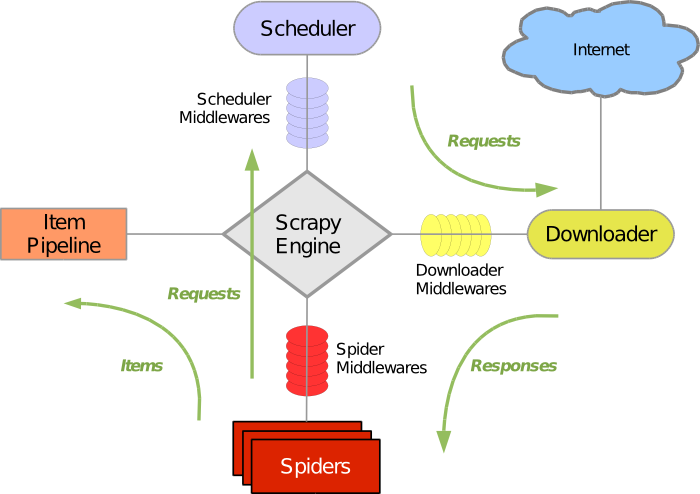
\includegraphics[scale=1]{scrapy_architecture.png}
	\caption{Visão geral da arquitetura do scrapy \cite{scrapy_arch}}
	\label{scrapy_architecture}
\end{figure}

\subsubsection{Scrapy engine}
\index{Scrapy!Arquitetura!Scrapy engine}

O engine é responsável por controlar o fluxo de dados entre todos os componentes do sistema, e disparar eventos quando certas ações ocorrerem.
% colocar mais informações sobre data flow

\subsubsection{Scheduler}
\index{Scrapy!Arquitetura!Scheduler}

O scheduler recebe requisições do engine e as enfileira para realimentação da engine no futuro.

\subsubsection{Downloader}
\index{Scrapy!Arquitetura!Downloader}

O Downloader é responsável por obter páginas da Web e alimetar o engine, que por sua vez alimenta os crawlers/spiders.

\subsubsection{Item pipeline}
\index{Scrapy!Arquitetura!Item pipeline}

O Item Pipeline é responsável para processar os itens uma vez que eles foram extraídos pelos crawlers/spiders. Tarefas típicas do Item Pipeline incluem limpeza, validação e persistência do item.

%colocar mais informações sobre o este item

\subsubsection{Spider middlewares}
\index{Scrapy!Arquitetura!Spider middlewares}

Spider middlewares são \emph{ganchos} específicos que ficam entre a Engine e os Spiders e podem processar a entrada de um sipder (respostas) e saídas (itens e requisições). Eles fornecem um mecanismo conveniente para estender as funcionalidades do Scrapy através da adição de código customizado.

%colocar mais informações sobre o spider middleware

\subsubsection{Scheduler middlewares}
\index{Scrapy!Arquitetura!Scheduler middlewares}

Scheduler middlewares são \emph{ganchos} específicos que ficam entre a Engine e o Schedule e processa requisições quando as mesmas passam do engine para o Scheduler e vice-versa. Eles fornecem um mecanismo conveniente para estender as funcionalidades do Scrapy através da adição de código customizado.

\subsubsection{Fluxo de dados}
\index{Scrapy!Arquitetura!Fluxo de dados}

O fluxo de dados do Scrapy é controlado pela Engine e funciona da seguinte forma:

\begin{enumerate}
	\item Engine abre um domínio, localiza o Spider que manipula aquele domínio e pede para o Spider a primeira URL para navegar.
	\item O Engine pega a primeira URL para navegar do Spider e a agenda no Scheduler como Requisições.
	\item O Engine pede para o Scheduler as próximas URLs para navegar.
	\item O Scheduler retorna a próxima URL para navegação para o Engine e o Engine a manda para o Downloader passando pelo Downloader Middleware.
	\item Uma vez que o download da página terminou, o Downloader gera uma Response (com a página) e a manda para o Engine, passando pelo Downloader Middleware.
	\item O Engine recebe a resposta do downloader e a envia para o Spider processar, passando pelo Spider Middleware.
	\item O Spider processa a Response e retorna os itens obtidos e novas Requests para o Engine.
	\item O Engine envia os itens obtidos (retornados pelo spider) para o Item Pipeline e envia as Requests (retornadas pelo Spider) para o Scheduler.
	\item O processo se repete a partir do passo 2 até que não haja mais Requests no Scheduler e o Engine fecha o domínio.
\end{enumerate}

\subsubsection{E/S orientado a eventos}
\index{Scrapy!Arquitetura!Networking orientado a eventos}

O Scrapy é escrito utilizando o Twisted \cite{twisted}, um framework popular para programação orientada a eventos para Python. Desta forma, ele é implementado utilizado código não-bloqueante (ou assíncrono) para aumentar a concorrência.

\subsection{Serviços embutidos}
\index{Scrapy!Serviços embutidos}

O Scrapy possui uma gama de serviços embutidos feitos para facilitar a monitoração e manutenção do sistema. A seguir, é apresentado cada um destes serviços embutidos bem como uma descrição breve.

\subsubsection{Logging}
\index{Scrapy!Serviços embutidos!Logging}

O log é um histórico de execução do sistema. Através da análise de logs, é possível detectar e achar a fonte de problemas. O Scrapy possui um componente de logging que grava as mensagens de log em um arquivo em disco e possui cinco níveis de log \cite{scrapy_log}:

\begin{enumerate}
	\item \texttt{\textbf{CRITICAL}} - Para erros críticos
	\item \texttt{\textbf{ERROR}} - Para erros regulares
	\item \texttt{\textbf{WARNING}} - Para avisos
	\item \texttt{\textbf{INFO}} - Para mensagens informativas
	\item \texttt{\textbf{DEBUG}} - Para mensagens de debug
\end{enumerate}

O nível de log é configurável e um determinado nível irá catalogar todas as mensagens do nível mais as mensagens dos níveis abaixo. Por exemplo, se o nível de log for configurado para 5 (\texttt{DEBUG}), o sistema irá gravar todas as mensagens de log, ao passo que se o nível de log for configurado para 2 (\texttt{ERROR}), somente as mensagens de erros regulares e erros críticos serão gravados.



\pagebreak
\section{Website Parse Template}
\index{Website Parse Template}


Website Parse Template (WPT) é um formato aberto baseado em XML que fornece informações adicionais a web crawlers como estrutura e conteúdo do HTML. O WPT é compatível com esquemas XML, como o RDF e o OWL \cite{wpt}. É composto por três seções principais:

\begin{itemize}
	\item \textbf{Templates} - Seção mandatória, que contém descrições sobre estrutura e conteúdo de páginas da web em HTML.
	\item \textbf{Ontologia} - Seção opcional que define conceitos e relações usadas em um website.
	\item \textbf{URLs} - Seção opcional, que associa certos padrões de URL para grupos de páginas web para templates específicos. 
\end{itemize}

Cada uma das seções do WPT mostradas acima será discutida a seguir.

\subsection{Seções do WPT}
\index{Website Parse Template!Seções do WPT}

\subsubsection{Templates}
\index{Website Parse Template!Seções do WPT}

A seção de templates descreve a estrutura do HTML fazendo referências aos elementos HTML correspondentes da página em específico \cite{wpt}.

O Template inicia com a tag \texttt{<ow:template>} e termina com  \texttt{</ow:template>}. É obrigatório especificar um nome de template único dentro da tag \texttt{<ow:template>} e definir a URL correspondente ao template específico.

O Template é composto de blocos correspondentes a cada elemento estrutural de uma página web em específico. Cada template precisa ter ao menos um bloco. Um bloco faz referência ao elemento HTML apropriado através de uma ou muitas combinações dos seguintes métodos de referência: TagID, XPath e Pattern. Cada bloco precisa iniciar com uma tag \texttt{<ow:block>} e fechar com \texttt{</ow:block>}. É necessário indicar elementos HTML específicos dentro da tag de abertura do bloco.

\pagebreak
\lstset{language=XML,
basicstyle=\scriptsize,
caption={Exemplo de um Template com três blocos \cite{wpt}},
captionpos=b
}
\begin{lstlisting}
<ow:template ow:name="Template Example" ow:url="http://www.example.com/index.php">
  <ow:block ow:tagid="ex1" ow:xpath="/html/body/div/div" ow:pattern="content (object[[a-z]*])">
    <!--descricao do conteudo -->
  </ow:block>
  <ow:block ow:tagid="ex2">
    <!-- descricao do conteudo -->
  </ow:block>
  <ow:block ow:xpath="/html/body/div/div/table/tr[1]/td">
    <!-- descricao do conteudo -->
  </ow:block>
</ow:template>
\end{lstlisting}

Cada bloco contém o a descrição do conteúdo dos elementos HTML representados isoladamente ou dentro de outro bloco. Blocos embutidos são usados para descrever elementos HTML específicos ("bloco pai") que inclui um ou mais elementos ("bloco filho").

\lstset{language=XML,
basicstyle=\scriptsize,
caption={Exemplo de um Template com blocos embutidos \cite{wpt}},
captionpos=b
}
\begin{lstlisting}
<ow:template ow:name="Template Example" ow:url="http://www.example.com/index.php">

  <ow:block ow:xpath="/html/body/div/div">
    <ow:block ow:xpath="/html/body/div/div/table/tbody/tr[1]/td">
      <!-- descricao do conteudo -->
    </ow:block>
  </ow:block>
  
</ow:template>
\end{lstlisting}

A descrição do conteúdo pode ser informada usando conceitos definidos na seção \emph{Ontology} ou qualquer linguagem/formato suportado: RDF, CWL, etc. É necessário declarar namespaces dos schemas XML usados dentro da tag \texttt{<ow:wpt>} e o nome da ontologia dentro da tag \texttt{<ow:template>}

\pagebreak
\lstset{language=XML,
basicstyle=\scriptsize,
caption={Exemplo de um Template com instâncias de descrição de conteúdo\cite{wpt}},
captionpos=b
}
\begin{lstlisting}
<ow:wpt xmlns:ow="http://www.omfica.org/schemas/ow/0.9"
 xmlns:rdf="http://www.w3.org/1999/02/22-rdf-syntax-ns#"
 ow:host="http://www.example.com">

  <ow:template ow:name="Template Example" ow:url="http://www.example.com/index.php"
   ow:ontology="ontology_example">

     <!-- descricao de conteudo utilizando conceitos definidos -->
     <ow:block ow:tagid="ex1" ow:xpath="/html/body/div/div" ow:pattern="Wellcome (user.name[[A-Za-z]*])">
       conceito_de_ontologia
     </ow:block>
     <!-- descricao de conteudo utilizando a sintaxe RDF -->
     <ow:block ow:tagid="ex2">
       <rdf:Description rdf:about="http://www.example.com/index.php">
       </rdf:Description>
     </ow:block>
     <!-- descricao de conteudo utiliznado CWL.unl -->
     <ow:block ow:xpath="/html/body/div/div/table/tr[1]/td">
       {cwl.unl}
       {/cwl.unl}
     </ow:block>
  </ow:template>

</ow:wpt>
\end{lstlisting}

\subsubsection{URLs}
\index{Website Parse Template!URLs}

Esta seção define as URLS/padrões de URLs das páginas web descritas na seção de Templates. Esta seção é mandatória se os templates não definem as URLs/padrões de URL das páginas web \cite{wpt}.

De acordo com a seção de Templates, esta seção também pode consistir de vários blocos/unidades. Cada um destes blocos iniciam com a tag \texttt{<ow:urls>} e terminam com a tag \texttt{</ow:urls>}.


\lstset{language=XML,
basicstyle=\scriptsize,
caption={Exemplo de padrões de URLs \cite{wpt}},
captionpos=b,
label="wpt_url_pattern"
}
\begin{lstlisting}
\label{lst:wpt_url_pattern}
<ow:urls ow:name="Artist page on Yahoo! Music" ow:template="Artist page on Yahoo! Music">
  <ow:url>http://music.yahoo.com/ar-8206256---Amy-Winehouse</ow:url>
  <ow:url>http://music.yahoo.com/ar-([artist.id[0-9]*])---(artist.name[[A-Za-z0-9-]*])</ow:url>
</urls>
\end{lstlisting}

Especificações utilizando expressões regulares (RegExp) são utilizadas para descrição de padrões de URL. O padrão de URL informado na listagem 1.4 também inclui a real URL representada. Os conceitos necessários para definição de padrões de URL (tais como "id" e "nome") são definidos na seção Ontology.

\subsubsection{Ontology}
\index{Website Parse Template!URLs}

\pagebreak
\section{Protocol Buffers}
\index{Protocol Buffers}

% justificativa
\chapter{Justificativa}

Recuperação de Informações na Web é uma tarefa fácil, porém trabalhosa se feita manualmente por humanos. Fácil, pois conseguimos detectar padrões de informações, categoriza-las e armazena-las como quisermos. Trabalhosa, pois podem haver inúmeras páginas com grandes quantidades de informação, o que torna o processo de recuperação manual de informações caro, trabalhoso e tedioso.

Soluções computacionais como \emph{web crawlers} ou \emph{web scrapers} ajudam na automação do processo de recuperação de informações estruturadas. 

No entanto, por serem soluções computacionais, demandam que sejam programadas e, geralmente, para um fim específico. Um \emph{web scraper} que foi originalmente desenvolvido para extrair informações de um determinado tipo de página, não conseguirá extrair as mesmas informações se a estrutura e/ou organização da página mudarem.

Na prática, um \emph{web scraper} projetado para um sítio, precisará sofrer modificações de forma que consiga extrair informações caso a estrutura da página em HTML mude, seja por uma mudança na estrutura de páginas do sítio ou pelo uso de um novo sítio que possa prover as mesmas informações.

Com a recuperação de informações de forma manual, havia o problema da falta de automação de processo, o que pode levar a um alto custo humano de recuperação de informações. Com a automação do processo, pode haver o problema de alto custo de criação e manutenção dos softwares responsáveis pela recuperação de informação estruturada.

O presente trabalho visa criar um método que diminua os custos de criação e manutenção de \emph{web scrapers} por meio da criação automatizada destes softwares através do uso de \emph{templates} em XML.
% objetivos
\chapter{Objetivos}
\thispagestyle{fancy}

\section{Objetivo Geral}

Facilitar a criação de sistemas para recuperação de informações estruturadas na Web através do uso de templates em XML.

\section{Objetivos específicos}

\begin{enumerate}
	\item Diminuir os custos de criação e manutenção de sistemas para recuperação de informação estruturada na Web.
	\item Contribuição com projetos de código aberto.
\end{enumerate}
% metodologia
\chapter{Metodologia}

A elaboração do presente trabalho se deu em 3 etapas distintas:

\begin{enumerate}
	\item Estudo de viabilidade do \emph{Website Parse Template} (WPT) como \emph{Domain Specific Language} (DSL) para \emph{web scrapers}, assim como busca de melhores alternativas.
	\item Estudo do funcionamento e arquitetura do framework Scrapy.
	\item Implementação de um protótipo e seus respectivos testes automatizados para compilação do WPT em um \emph{spider} do Scrapy.
\end{enumerate}

A seguir, é mostrada uma descrição mais detalhada de cada etapa de produção deste trabalho.

\section{Estudo de viabilidade do WPT e outras alternativas}

Uma preocupação constante no desenvolvimento do presente trabalho foi a procura por adoção de padrões abertos, que sejam amplamente utilizados e que não representem um gargalo durante o desenvolvimento.

Além do Website Parse Template, outras duas alternativas foram pesquisadas: o Protocol Buffer \cite{protobuf} e o JSON \cite{JSON}. Ambas foram descartadas pelos motivos citados anteriormente ao passo que o WPT se encaixou bem na lista de requisitos.

\section{Estudo do Scrapy}

Uma das grandes vantagens percebidas do framework Scrapy é a sua abundante documentação, seja a oficial em documentos HTML ou a documentação disponível dentro do próprio código fonte do mesmo.

Os principais itens estudados foram a geração de código, comandos disponíveis na linha de comando, testes unitários automatizados e estratégias de desenvolvimento.

O Scrapy possui uma coleção de testes automatizados, que permitem um melhor entendimento do framewok ao observar o que e como os componentes do mesmo estão sendo testados. Além disso, os testes disponíveis fornecem um esquema pré-definido de como os testes para novas funcionalidades deverão ser feitos. Os testes deste protótipo se encontram no pacote \texttt{scrapy.tests.test\_commands}, ao passo que sua implementação se encontra em \texttt{scrapy.commands.importwpt}.

\section{Desenvolvimento do protótipo}

O Scrapy possui um utilitário de linha de comando que permite a criação de novos projetos de \emph{web scrapers}, assim como sua execução, manutenção e observação de funcionamento do projeto. O exemplo a seguir ilustra a saída da execução do comando "scrapy":

\lstset{basicstyle=\scriptsize,
caption={Saída da execução do comando ''scrapy''},
captionpos=b
}
\begin{lstlisting}
Scrapy 0.11 - no active project

Usage:
  scrapy <command> [options] [args]

Available commands:
  fetch         Fetch a URL using the Scrapy downloader
  runspider     Run a self-contained spider (without creating a project)
  settings      Get settings values
  shell         Interactive scraping console
  startproject  Create new project
  version       Print Scrapy version
  view          Open URL in browser, as seen by Scrapy

Use "scrapy <command> -h" to see more info about a command
\end{lstlisting}

O protótipo desenvolvido neste trabalho foi incluído no comando apresentado anteriormente e pode ser observado quando o Scrapy detecta que está dentro de uma pasta de projeto:

\pagebreak
\lstset{basicstyle=\scriptsize,
caption={Saída da execução do comando ''scrapy'' dentro da pasta de um projeto},
captionpos=b
}
\begin{lstlisting}
Scrapy 0.11 - project: scrapytest

Usage:
  scrapy <command> [options] [args]

Available commands:
  crawl         Start crawling from a spider or URL
  deploy        Deploy project in Scrapyd server
  fetch         Fetch a URL using the Scrapy downloader
  genspider     Generate new spider using pre-defined templates
  importwpt     Create a spider based on a Website Parse Template (WPT) file
  list          List available spiders
  parse         Parse URL (using its spider) and print the results
  queue         Control execution queue
  runserver     Start Scrapy in server mode
  runspider     Run a self-contained spider (without creating a project)
  settings      Get settings values
  shell         Interactive scraping console
  startproject  Create new project
  version       Print Scrapy version
  view          Open URL in browser, as seen by Scrapy

Use "scrapy <command> -h" to see more info about a command

\end{lstlisting}

O comando \texttt{importwpt} cd lê um arquivo XML utilizando o formato WPT e cria um \emph{spider} do scrapy a partir dele. Após isso, a execução do comando \texttt{scrapy crawl nome\_do\_spider\_gerado} irá executar o processo de extração de informações conforme descrito no XML que foi importado.

Dentre todos os elementos e seus atributos que a especificação do WPT apresenta, não há nenhum que diz sobre o tratamento e armazenamento dos dados obtidos. Por este motivo, somente a especificação do WPT é insuficiente para construir um sistema de recuperação de informações completo. Por exemplo, o atributo não-oficial \texttt{name} dentro da tag \texttt{<ow:block>} é necessário para nomeação de objetos dentro do \emph{spider}:

\lstset{language=XML,
basicstyle=\scriptsize,
caption={Conteúdo do arquivo de entrada para o comando \texttt{scrapy importwpt}},
captionpos=b
}
\begin{lstlisting}
  <ow:wpt xmlns:ow="http://www.omfica.org/schemas/ow/0.9"
            ow:host="http://example.com">
  <ow:template ow:name="Template Example" ow:url="http://www.example.com/index.php">
      <ow:block ow:tagid="ex1" name="ex1"></ow:block>
  </ow:template> 
  </ow:wpt>
\end{lstlisting}

Como o principal objetivo deste trabalho é facilitar a criação e manutenção de sistemas de recuperação de informação, não é desejável ter nomes de variáveis geradas aleatoriamente no processo de conversão do WPT para o spider do Scrapy. Observa-se, então, o uso do conteúdo do atributo \texttt{name} no código gerado:

\lstset{language=Python,
basicstyle=\scriptsize,
caption={\emph{Spider} gerado a partir do arquivo de entrada apresentado na listagem 5.3},
captionpos=b
}
\begin{lstlisting}
from scrapy.item import Item, Field

class TemplateExampleItem1(Item):
    ex1 = Field()

from scrapy.spider import BaseSpider
from scrapy.contrib.loader import XPathItemLoader

class TemplateExample(BaseSpider):
    name = 'example.com'
    allowed_domains = ['example.com']
    start_urls = [
        'http://www.example.com/index.php',
    ]

    def parse(self, response):
        l = XPathItemLoader(item = TemplateExampleItem1(),response=response)
        l.add_xpath('bubble','id("ex1")/text()') 
        i = l.load_item()
        yield i

\end{lstlisting}


Como este trabalho ainda está em andamento, algumas funcionalidades, tais como exportação dos dados obtidos, não estão presentes. Por ser um projeto de código aberto, há a possibilidade deste protótipo ser desenvolvido por outras pessoas e mais funcionalidades serem adicionadas com o passar do tempo.

No entanto, no que tange á criação de \emph{spiders}, o projeto funciona conforme as especificações do WPT (disponíveis em \cite{wpt}). Como estas especificações ainda estão em desenvolvimento, é possível que em um futuro próximo seja necessária a manutenção do projeto a fim de ser compatível com a última versão do WPT.
% resultados.tex
\chapter{Resultados}

O protótipo aqui apresentado ainda encontra-se em desenvolvimento. Por ser uma contribuição ao Scrapy, um framework de código aberto, este protótipo poderá ser desenvolvido por outros membros da comunidade.

Um dos aspectos positivos da abordagem adotada é que a ferramenta desenvolvida gera código na linguagem de programação Python a partir de código em XML, permitindo que o programador faça altarações no código gerado, caso seja necessário. 

Como este trabalho não contempla, tampouco pretende contemplar, todas as facetas da criação de sistemas de recuperação de informações estruturadas na Web, a possibilidade do programador alterar o código gerado pode vir a ser bem útil em situações mais específicas. Por isso o objetivo deste trabalho é \emph{gerar código} ao invés de \emph{interpretar código} com o intuito de criar sistemas de recuperação de informações.

Pelo fato dos objetivos deste trabalho se basearem na criação de uma ferramenta que facilite a criação de sistemas de recuperção de informação na Web, duas análises podem ser feitas com os resultados: uma quantitativa e outra qualitativa. Quantitativa para mostrar as visíveis economias no processo de escrita/manutenção de código. Qualitativa para mostrar como os resultados obtidos podem levar a uma maior produtividade, menor curva de aprendizado e resultados mais rápidos. Também se faz necessária a demonstração de exemplos de sistemas de recuperação de informações reais criados a partir do uso da abordagem desenvolvida neste trabalho, bem como as dificuldades encontras e trabalhos futuros.

A seguir, duas avaliações são mostradas, quantitativas e qualitativas, dos resultados obtidos. Logo a seguir, há exemplos de spiders reais gerados a partir da ferramenta, dificuldades encontradas e trabalhos futuros.

\section{Avaliação quantitativa}

A avaliação de sucesso no cumprimento dos objetivos deste projeto pode ser meramente subjetiva, porém, há alguns critérios quantitativos ou subjetivos que podem ser discutidos, como a economia em linhas de código. No exemplo mais simples possível, há o seguinte template:

\lstset{language=XML,
basicstyle=\scriptsize,
caption={Exemplo de template em WPT},
captionpos=b
}
\begin{lstlisting}
  <ow:wpt xmlns:ow="http://www.omfica.org/schemas/ow/0.9"
            ow:host="http://example.com">
  <ow:template ow:name="Template Example" ow:url="http://www.example.com/index.php">
      <ow:block ow:tagid="ex1" name="ex1"></ow:block>
  </ow:template> 
  </ow:wpt>
\end{lstlisting}

O template anterior gera o seguinte código em Python:

\lstset{language=Python,
basicstyle=\scriptsize,
caption={\emph{Spider} gerado a partir do arquivo de entrada apresentado na listagem 5.3},
captionpos=b
}
\begin{lstlisting}
from scrapy.item import Item, Field

class TemplateExampleItem1(Item):
    ex1 = Field()

from scrapy.spider import BaseSpider
from scrapy.contrib.loader import XPathItemLoader

class TemplateExample(BaseSpider):
    name = 'example.com'
    allowed_domains = ['example.com']
    start_urls = [
        'http://www.example.com/index.php',
    ]
    
    def parse(self, response):
        l = XPathItemLoader(item = TemplateExampleItem1(),response=response)
        l.add_xpath('bubble','id("ex1")/text()') 
        i = l.load_item()
        yield i
\end{lstlisting}

O código em Python possui 20 linhas, 16 sem as linhas em branco, ao passo que o template possui apenas 5 linhas de código. Neste exemplo, na pior das hipóteses, a economia de código gira em torno de 2/3 do original. A diferença fica mais evidente em um exemplo mais completo:

\lstset{language=XML,
basicstyle=\scriptsize,
caption={Exemplo mais completo de template em WPT},
captionpos=b
}
\begin{lstlisting}
<ow:wpt xmlns:ow="http://www.omfica.org/schemas/ow/0.9"
ow:host="http://example.com">
<ow:template ow:name="Template Example" ow:url="http://www.example.com/index.php">
  <ow:block ow:tagid="ex1" name="ex1"></ow:block>
  <ow:block ow:xpath="/html/body/p/text()" name="paragraph"></ow:block>
  
  <ow:block ow:xpath="/html/body/ul/li" name="menu">
    <ow:block ow:xpath="//a/text()" name="item" ow:type="repetable"></ow:block>
    <ow:block ow:xpath="//a[@href]" name="url" ow:type="repetable"></ow:block>
  </ow:block>
  
  <ow:block ow:xpath="/html/body/div[2]/ul/li" name="paginate">
    <ow:block ow:xpath="//a[@href]" name="url" ow:type="follow"></ow:block> <!-- follow -->
  </ow:block>
</ow:template> 
</ow:wpt>
\end{lstlisting}

\pagebreak
\lstset{language=Python,
basicstyle=\scriptsize,
caption={\emph{Spider} gerado a partir do arquivo de entrada apresentado na listagem 5.3},
captionpos=b
}
\begin{lstlisting}
from scrapy.item import Item, Field

class TemplateExampleItem1(Item):
    ex1 = Field()

class TemplateExampleItem2(Item):
    paragraph = Field()
    
class MenuItem(Item):
    item = Field()
    url = Field()
    
class Paginate(Item):
    url = Field()

from scrapy.spider import BaseSpider
from scrapy.contrib.loader import XPathItemLoader
from scrapy.selector import HtmlXPathSelector
from scrapy.http import Request

class TemplateExample(BaseSpider):
    name = 'example.com'
    allowed_domains = ['example.com']
    start_urls = [
        'http://www.example.com/index.php',
    ]

    def parse(self, response):
        l = XPathItemLoader(item = TemplateExampleItem1(),response=response)
        l.add_xpath('bubble','id("ex1")/text()') 
        i = l.load_item()
        yield i
        
        l = XPathItemLoader(item = TemplateExampleItem2(),response=response)
        l.add_xpath('paragraph','/html/body/p/text()') 
        i = l.load_item()
        yield i
        
        hxs = HtmlXPathSelector(response)
        for item in hxs.select('/html/body/ul/li'):
            l = XPathItemLoader(item = MenuItem(), selector=item)
            l.add_xpath('item','//li/a/text()') 
            l.add_xpath('url','//li/a[@href]') 
            i = l.load_item()
            yield i
                        
        hxs = HtmlXPathSelector(response)
        for item in hxs.select('/html/body/div[2]/ul/li'):
            l = XPathItemLoader(item = Paginate(), selector=item)
            l.add_xpath('url','//li/a[@href]') 
            i = l.load_item()
            yield Request(item=i['url'],callback=self.parse)
            yield i
\end{lstlisting}

Neste segundo exemplo, o arquivo XML possui 15 linhas, ao passo que o código gerado possui cerca de 60 linhas, aproximadamente 4 vezes menos código.

\pagebreak
\section{Avaliação qualitativa}

Em uma comparação qualitativa, pode-se citar alguns critérios:

\begin{enumerate}
	\item Linguagens de propósito geral \emph{versus} linguagens de proposíto específico (ou Domain Specific Languages).
	\item Ganho de produtividade.
	\item Facilidade para o usuário final.
	\item Automação de processos.
\end{enumerate}

Linguagens de propósito geral servem para construção de mais diversos tipos de sistemas, ao passo que linguagens de propósito específico são projetadas para resolver problemas em um domínio específico. Há um \emph{tradeoff} entre as duas abordagens: enquanto as linguagens de propósito geral são mais completas, elas também são mais complexas se comparadas com as linguagens de propósito específico para a mesma categoria de problema.

Quando se deixa de usar uma linguagem de propósito geral (Python) para utilizar outra de propósito específico (XML/WPT) o ganho de produtividade estará em eliminar preocupações não inerentes ao domínio. Com menos recursos e preocupações para se trabalhar, o trabalho do usuário final é facilitado.

Por exemplo, quando se trabalha com uma linguagem de propósito geral (como Python, C/C++ ou Java), o programador dispõe de uma maior flexibilidade, pois o mesmo pode valer de estruturas de controle, repetição, variáveis, funções ou métodos, classes, objetos, interação com o sistema de arquivos e E/S, interação com outros sistemas e tratamento de exceções para desenvolver suas soluções. Além de todos os itens relacionados à linguagem de programação, o programador precisa ter domínio de técnicas de extração de informações de páginas na Web, em que, nos casos mais simples envolve o conhecimento de uma linguagem de marcação (HTML, por exemplo), bibliotecas utilizadas para \emph{parsing} e bibliotecas para comunicação com servidores HTTP (\emph{HyperText Transfer Protocol} - Protocolo de Transferência de HiperTexto). No caso de uma linguagem específica de domínio baseada em XML, o programador precisará ter as mesmas noções de extração de informações de páginas na Web, porém sem a complexidade de lidar com uma linguagem de propósito geral e todas as suas respectivas dependências (bibliotecas), limitando-se apenas a conhecer a sintaxe do XML e as regras inerentes ao WPT.

O uso de XML pode trazer várias vantagens à criação de sistemas de recuperação de informação. A principal é que qualquer linguagem de programação que dê suporte à XML pode criar templates. Como o trabalho de \emph{não} escrever código é sempre menor do que escrever \emph{algum} código, os usuários podem se beneficiar com a criação de sistemas que geram templates automaticamente. Por exemplo, um \emph{plugin} de um navegador Web pode permitir que o usuário selecione as seções de uma determinada página que gostaria que fossem recuperadas automaticamente e então gerar o template para o mesmo.

\section{Exemplos reais}

\pagebreak
\section{Dificuldades encontradas}

Apesar da abundante documentação e mesmo não possuindo uma má qualidade de código ou baixa cobertura de testes, uma das principais dificuldades foi aderir à arquitetura e estilo de codificação do Scrapy para que a padronização entre componentes fosse mantida.

O framework em si possui um tamanho considerável (759 arquivos em 13/11/2010 \footnote{Informação obtida através do comando \texttt{find | wc -l} }), portanto, leva-se um tempo para acostumar-se com a estrutura de diretórios, arquivos e padrões de nome.

Não foi possível encontrar referências acadêmicas do Scrapy, um dos motivos pelos quais somente a respectiva documentação oficial foi utilizada.

O formato WPT possui apenas informações sobre a disposição dos elementos em uma página e seus respectivos significados (ontologia). Tal fato leva ao incoveniente de haver diferentes \emph{schemas} XML em um mesmo arquivo para determinar outras informações, como nome dos variáveis do código gerado e formato de persistência dos dados obtidos.

A biblioteca padrão para testes disponíveis no Python 2.6 (utilizado neste trabalho), a \texttt{unittest}, não possui um método de comparação de strings linha-a-linha. Isso significa que, se um texto precisa ser comparado com outro em um teste unitário, os dois serão comparados em sua totalidade, não linha-a-linha. 

Esta dificuldade torna os testes de geração de código mais trabalhosos, pois é necessário observar cada caractere com cautela quando os dois textos, o esperado e o obtido, falham no teste unitário.

Outra dificuldade encontrada nos testes unitários foi o teste de comandos, devido ao tempo que os testes levam para serem executados. A suíte de testes do Scrapy levam aproximadamente 30 segundos para serem executados\footnote{Os testes são executados com o comando \texttt{bin/runtests.sh scrapy.tests} dentro do diretório raiz do código fonte do Scrapy }, o que atrasa o desenvolvimento, já que a cada modificação no código, os testes precisam ser executados.

\pagebreak
\section{Trabalhos futuros}

O atual sistema ainda possui algumas limitações, como a falta de persistência dos dados obtidos. No atual cenário, é necessário que o programador altere o código fonte gerado para que os itens gerados pelo Scrapy durante a recuperação de informações sejam persistidos em disco.

O presente trabalho conseguiu atingir o objetivo de facilitar a criação e manutenção de sistemas de recuperação estruturada na Web, porém é possível facilitar ainda mais este trabalho. Plugins para navegadores Web podem ser criados de forma que os usuários possam criar os Website Parse Templates (WPT) através de uma interface visual.

Como o significado dos dados obtidos (metadados) não fazem parte deste trabalho, a seção \texttt{<ow:ontology>} do WPT é deliberadamente ignorada. Em trabalhos futuros, é provável que a mesma seja utilizada e então o protótipo aqui criado terá de ser modificado. 

\emph{Plugins} como o Firebug \cite{firebug} para o navegador Mozilla Firefox permitem inspecionar a estrutura do conteúdo de sítios na Web. Com ele, é possível selecionar elementos, mudar estilos e conteúdo, analisar o tráfego utilizado pelo acesso ao sítio e \emph{debugar} JavaScript. Usando o Firebug como plataforma, é possível desenvolver um outro complemento que facilite a criação de templates, o que poderia facilitar ainda mais o trabalho de criação de sistemas de recuperção de informações na Web.
% apendice.tex
\appendix
\chapter{Arquivos fonte}

\lstset{language=Python,
basicstyle=\scriptsize,
caption={Arquivo fonte do comando gerado para o Scrapy, o \texttt{importwpt.py}}
}
\begin{lstlisting}

from scrapy.command import ScrapyCommand
from scrapy.utils.misc import load_object
from scrapy.conf import settings
from scrapy.exceptions import UsageError
from scrapy import log
from lxml import objectify
from lxml.etree import XMLSyntaxError
import re
import sys
import string

XMLNS = '{http://www.omfica.org/schemas/ow/0.9}' 

spider_template = """from scrapy.spider import BaseSpider
from scrapy.contrib.loader import XPathItemLoader

class ${spider_class}(BaseSpider):
    name = ${name}
    allowed_domains = [${name}]
    start_urls = [${start_urls}]

    def parse(self, response):
        ${item_load}
"""

item_template = """
class ${item}(Item):
    ${fields}
"""

field_template="    ${field}=Field(${default})"

item_load_template = """l = XPathItemLoader(item = TemplateExampleItem1(),response=response)
        l.add_xpath('bubble','id("ex1")/text()') 
        i = l.load_item()"""


wpt_url = "http://www.w3.org/Submission/WPT/"

log.start()

class Command(ScrapyCommand):
    """
    Do a import of a WPT file 
    """
    requires_project = True

    def syntax(self):
        return "<file.xml>"

    def short_desc(self):
        return "Create a spider based on a Website Parse Template (WPT) file"

    def add_options(self, parser):
        ScrapyCommand.add_options(self, parser)

    def run(self, args, opts):

        if len(args) != 1:
            raise UsageError()

        filename = args[0]

        try:
            template = open(filename).read()

            root = objectify.fromstring(template)
            if not self._check_if_wpt_file_has_valid_url(root):
                log.msg("ERROR: attribute 'host' of 'wpt' tag does not have a valid URL",log.ERROR)

            if not self._check_if_wpt_has_at_least_one_template_with_one_block(xml):
                log.msg("ERROR: The WPT file must have at least one template tag\
                        with one block tag. See %s for more info" % wpt_url,log.ERROR);
    
            if not self._check_if_every_template_has_at_least_one_block(xml):
                log.msg("ERROR: Every template tag must have at least one block tag",log.ERROR)
    
            if not self._check_if_every_block_has_at_least_one_html_element_reference(xml):
                log.msg("ERROR: Every block tag must have at least one \
                        specific HTML tag reference (tagid, pattern or xpath).\
                        See %s for more info" % wpt_url,log.ERROR)

            if not self._check_if_every_template_has_a_unique_name(xml):
                log.msg("ERROR: Each template's name must be unique")
            
            if not self._check_if_url_section_is_valid_if_templates_has_no_urls(xml):
                log.msg("ERROR: Every template which does not have an 'ow:url'\
                        attribute must declare it in urls section. \
                        See %s for more info" % wpt_url,log.ERROR )

        except XMLSyntaxError,e:
            log.msg("ERROR: There is a markup error in %s" %filename,log.ERROR)
        except:
            log.msg("ERROR: File not found: %s" % filename,log.ERROR)
       
    def _check_if_wpt_file_has_valid_url(self,xml):
        try:
            url = xml.attrib[XMLNS+'host']
            p = re.compile('https?://([-A-Za-z0-9+&@#/%?=~_()|!:,.;]*[-A-Za-z0-9+&@#/%=~_()|])')
            domains = p.findall(url)
            
            if not domains: 
                return False
    
     
            domain = domains[0]

            self.domain = domain 

            if domain.__contains__('/'):
                domain = domain.split('/')[0]
     
            site_name = domain.split('.')[0]
     
            if site_name == 'www':
                site_name = domain.split('.')[1]

            self.site_name = site_name

        except:
            return False
    
        return True

    def _check_if_every_block_has_at_least_one_html_element_reference(self,xml):
        for t in xml.template:
            if not _check_if_every_block_has_at_least_one_html_element_reference(t.block):
                return False

        return True
   
    def _check_if_block_has_at_least_one_html_element_reference(self,block):
        if hasattr(block,'block'): 
            if not self._check_if_block_has_at_least_one_html_element_reference(block.block):
                return False

        for b in block:
            has_xpath = b.attrib.__contains__(XMLNS+'xpath')
            has_tagid = b.attrib.__contains__(XMLNS+'tagid')
            has_pattern = b.attrib.__contains__(XMLNS+'pattern')
            if not (has_xpath or has_tagid or has_pattern):
                return False

        return True
 
    def _check_if_every_template_has_at_least_one_block(self,xml):
        try:
            for i in range(0,xml.template.__len__()):
                if not self._template_has_block(xml,i):
                    return False
        except AttributeError:
            return False
        return True

    def _check_if_wpt_has_at_least_one_template_with_one_block(self,xml):
        return self._template_has_block(xml,0)

    def _template_has_block(self,xml,template_id):
        try:
            return hasattr(xml.template[template_id],'block')
        except AttributeError:
            return False
   
    def _check_if_every_template_has_a_unique_name(self,xml):
        template_names = []
        for t in xml.template:
            if t.attrib[XMLNS+'name'] in template_names:
                return False
            template_names.append(t.attrib[XMLNS+'name'])

        return True
    def _check_if_url_section_is_valid_if_templates_has_no_urls(self,xml):
        for t in xml.template:
            if t.attrib.__contains__(XMLNS+'url'):
                continue

            name = t.attrib[XMLNS+'name']
            urls = [u for u in xml.urls if u.attrib[XMLNS+'template']==name]

            if  len(urls)==0:
                return False

        return True

    def generate_spider_from_wpt(self,xml):
        oxml = objectify.fromstring(xml)

        item = self.get_items_from_wpt(oxml)
        t = string.Template(spider_template)
        spider_class = oxml.template.attrib[XMLNS+'name'].replace(' ','')
        name = "'"+self.domain+"'"
        start_urls = "'"+oxml.template.attrib[XMLNS+'url']+"'"
        item_load = self.get_items_load_from_wpt(oxml) 

        py = t.substitute(spider_class=spider_class,name=name,start_urls=start_urls,item_load=item_load)
        
        py = item+"\n"+py
        return py
    
    def get_items_from_wpt(self,xml):
        items = "\nfrom scrapy.item import Item, Field\n"
        blocks = xml.template.block
        class_counter = 1
        item_class_prefix = xml.template.attrib[XMLNS+'name'].replace(' ','')

        for b in blocks:
            class_name = item_class_prefix+"Item"+str(class_counter) 
            class_counter += 1
            fields = "%s = Field()" % b.attrib['name']

            t = string.Template(item_template) 
            items += t.substitute(item=class_name,fields=fields) 
        return items

    def get_items_load_from_wpt(self,xml):
        blocks = xml.template.block
        class_counter = 1
        item_class_prefix = xml.template.attrib[XMLNS+'name'].replace(' ','')
        item_load = ""
        for b in blocks:
            class_name = item_class_prefix+"Item"+str(class_counter)
            class_counter += 1
            t = string.Template(item_load_template)

            if b.attrib.__contains__(XMLNS+'tagid'):
                xpath = 'id("%s")/text()' % b.attrib[XMLNS+'tagid']
            
            field_name = b.attrib['name']

            item_load += t.substitute(class_name=class_name,field_name=field_name,xpath=xpath)

        return item_load
\end{lstlisting}

%-------------------------------------%<-------------------------------

\pagebreak

\lstset{language=Python,
basicstyle=\scriptsize,
caption={Arquivo fonte dos testes automatizados para o comando gerado para o Scrapy. Arquivo \texttt{test\_commands.py}}
}
\begin{lstlisting}

from __future__ import with_statement

import sys
import os
import subprocess
from os.path import exists, join, dirname, abspath
from shutil import rmtree
from tempfile import mkdtemp

from twisted.trial import unittest

import scrapy


class ProjectTest(unittest.TestCase):
    project_name = 'testproject'

    def setUp(self):
        self.temp_path = mkdtemp()
        self.cwd = self.temp_path
        self.proj_path = join(self.temp_path, self.project_name)
        self.proj_mod_path = join(self.proj_path, self.project_name)
        self.env = os.environ.copy()
        self.env['PYTHONPATH'] = dirname(scrapy.__path__[0])

    def tearDown(self):
        rmtree(self.temp_path)

    def call(self, *new_args, **kwargs):
        out = os.tmpfile()
        args = (sys.executable, '-m', 'scrapy.cmdline') + new_args
        return subprocess.call(args, stdout=out, stderr=out, cwd=self.cwd, \
            env=self.env, **kwargs)

    def proc(self, *new_args, **kwargs):
        args = (sys.executable, '-m', 'scrapy.cmdline') + new_args
        return subprocess.Popen(args, stdout=subprocess.PIPE, stderr=subprocess.PIPE, \
            cwd=self.cwd, env=self.env, **kwargs)


class StartprojectTest(ProjectTest):

    def test_startproject(self):
        self.assertEqual(0, self.call('startproject', self.project_name))

        assert exists(join(self.proj_path, 'scrapy.cfg'))
        assert exists(join(self.proj_path, 'testproject'))
        assert exists(join(self.proj_mod_path, '__init__.py'))
        assert exists(join(self.proj_mod_path, 'items.py'))
        assert exists(join(self.proj_mod_path, 'pipelines.py'))
        assert exists(join(self.proj_mod_path, 'settings.py'))
        assert exists(join(self.proj_mod_path, 'spiders', '__init__.py'))

        self.assertEqual(1, self.call('startproject', self.project_name))
        self.assertEqual(1, self.call('startproject', 'wrong---project---name'))


class CommandTest(ProjectTest):

    def setUp(self):
        super(CommandTest, self).setUp()
        self.call('startproject', self.project_name)
        self.cwd = join(self.temp_path, self.project_name)
        self.env['SCRAPY_SETTINGS_MODULE'] = '%s.settings' % self.project_name


class GenspiderCommandTest(CommandTest):

    def test_arguments(self):
        # only pass one argument. spider script shouldn't be created
        self.assertEqual(2, self.call('genspider', 'test_name'))
        assert not exists(join(self.proj_mod_path, 'spiders', 'test_name.py'))
        # pass two arguments <name> <domain>. spider script should be created
        self.assertEqual(0, self.call('genspider', 'test_name', 'test.com'))
        assert exists(join(self.proj_mod_path, 'spiders', 'test_name.py'))

    def test_template(self, tplname='crawl'):
        args = ['--template=%s' % tplname] if tplname else []
        spname = 'test_spider'
        p = self.proc('genspider', spname, 'test.com', *args)
        out = p.stdout.read()
        self.assert_("Created spider %r using template %r in module" % (spname, tplname) in out)
        self.assert_(exists(join(self.proj_mod_path, 'spiders', 'test_spider.py')))
        p = self.proc('genspider', spname, 'test.com', *args)
        out = p.stdout.read()
        self.assert_("Spider %r already exists in module" % spname in out)

    def test_template_basic(self):
        self.test_template('basic')

    def test_template_csvfeed(self):
        self.test_template('csvfeed')

    def test_template_xmlfeed(self):
        self.test_template('xmlfeed')

    def test_list(self):
        self.assertEqual(0, self.call('genspider', '--list'))

    def test_dump(self):
        self.assertEqual(0, self.call('genspider', '--dump=basic'))
        self.assertEqual(0, self.call('genspider', '-d', 'basic'))


class MiscCommandsTest(CommandTest):

    def test_crawl(self):
        self.assertEqual(0, self.call('crawl'))

    def test_list(self):
        self.assertEqual(0, self.call('list'))

class RunSpiderCommandTest(CommandTest):

    def test_runspider(self):
        tmpdir = self.mktemp()
        os.mkdir(tmpdir)
        fname = abspath(join(tmpdir, 'myspider.py'))
        with open(fname, 'w') as f:
            f.write("""
from scrapy import log
from scrapy.spider import BaseSpider

class MySpider(BaseSpider):
    name = 'myspider'

    def start_requests(self):
        self.log("It Works!")
        return []
""")
        p = self.proc('runspider', fname)
        log = p.stderr.read()
        self.assert_("[myspider] DEBUG: It Works!" in log)
        self.assert_("[myspider] INFO: Spider opened" in log)
        self.assert_("[myspider] INFO: Closing spider (finished)" in log)
        self.assert_("[myspider] INFO: Spider closed (finished)" in log)

    def test_runspider_no_spider_found(self):
        tmpdir = self.mktemp()
        os.mkdir(tmpdir)
        fname = abspath(join(tmpdir, 'myspider.py'))
        with open(fname, 'w') as f:
            f.write("""
from scrapy import log
from scrapy.spider import BaseSpider
""")
        p = self.proc('runspider', fname)
        log = p.stderr.read()
        self.assert_("No spider found in file" in log)

    def test_runspider_file_not_found(self):
        p = self.proc('runspider', 'some_non_existent_file')
        log = p.stderr.read()
        self.assert_("File not found: some_non_existent_file" in log)

    def test_runspider_unable_to_load(self):
        tmpdir = self.mktemp()
        os.mkdir(tmpdir)
        fname = abspath(join(tmpdir, 'myspider.txt'))
        with open(fname, 'w') as f:
            f.write("")
        p = self.proc('runspider', fname)
        log = p.stderr.read()
        self.assert_("Unable to load" in log)


class ImportWptCommandTest(CommandTest):

    def test_import_file_not_found(self):
        p = self.proc("importwpt","some_non_existent_file")
        log = p.stderr.read()
        self.assert_("ERROR: File not found: some_non_existent_file" in log,'Log contents: '+log)

    def test_import_existent_file_invalid_markup(self):
        tmpdir = self.mktemp()
        os.mkdir(tmpdir)
        fname = abspath(join(tmpdir,"mytemplate.xml"))
        open(fname,"w").write("")
        p = self.proc("importwpt",fname)
        log = p.stderr.read()

        self.assert_(("ERROR: There is a markup error in %s" % fname) in log,'Log contents: '+log)

    def _test_import_valid_markup_with_no_template_tag(self):
        tmpdir = self.mktemp()
        os.mkdir(tmpdir)
        fname = abspath(join(tmpdir,"mytemplate.xml"))
        
        xml = '<?xml version="1.0" encoding="UTF-8"?>\
                     <ow:wpt xmlns:ow="http://www.omfica.org/schemas/ow/0.9" \
                                ow:host="http://www.example.com"> \
                     </ow:wpt>'
        
        with open(fname,"w") as f:
            f.write(xml)
            p = self.proc('importwpt',fname)
            log = p.stderr.read()

        self.assert_("ERROR: The WPT file must have at least one template tag\
                        with one block tag." in log,"log contents %s" % log)

    def test_validate_business_rules(self):
        from lxml import objectify
        from scrapy.commands.importwpt import Command

        cmd = Command()
        
        "_check_if_wpt_file_has_valid_url"
        xml = '<ow:wpt xmlns:ow="http://www.omfica.org/schemas/ow/0.9"></ow:wpt>'
        
        oxml = objectify.fromstring(xml)
        check = cmd._check_if_wpt_file_has_valid_url(oxml)
        self.assert_(not check)
 
        xml = '<ow:wpt xmlns:ow="http://www.omfica.org/schemas/ow/0.9" \
                ow:host="http://example.com"></ow:wpt>'

        oxml = objectify.fromstring(xml)
        check = cmd._check_if_wpt_file_has_valid_url(oxml)
        self.assert_(check)

        "_check_if_wpt_has_at_least_one_template_with_one_block"
        
        check = cmd._check_if_wpt_has_at_least_one_template_with_one_block(oxml)
        self.assert_(not check)
        xml = '<ow:wpt xmlns:ow="http://www.omfica.org/schemas/ow/0.9" \
                ow:host="http://example.com">\
                <ow:template ow:name="Template Example" ow:url="http://www.example.com/index.php"> \
                    <ow:block></ow:block> \
                </ow:template> \
                </ow:wpt>'
        oxml = objectify.fromstring(xml)
        check = cmd._template_has_block(oxml,0) 
        self.assert_(check)

        check = cmd._check_if_wpt_has_at_least_one_template_with_one_block(oxml)
        self.assert_(check)
        
        "_check_if_block_has_at_least_one_html_element_reference"
        check = cmd._check_if_block_has_at_least_one_html_element_reference(oxml.template.block)
        self.assert_(not check)

        xml = '<ow:wpt xmlns:ow="http://www.omfica.org/schemas/ow/0.9" \
                ow:host="http://example.com">\
                <ow:template ow:name="Template Example" ow:url="http://www.example.com/index.php"> \
                    <ow:block ow:tagid="ex1"></ow:block> \
                </ow:template> \
                </ow:wpt>'

        oxml = objectify.fromstring(xml)
        check = cmd._check_if_block_has_at_least_one_html_element_reference(oxml.template.block) 
        self.assert_(check)

        xml = '<ow:wpt xmlns:ow="http://www.omfica.org/schemas/ow/0.9" \
                 ow:host="http://example.com">\
                 <ow:template ow:name="Template Example" ow:url="http://www.example.com/index.php"> \
                     <ow:block ow:tagid="ex1"> \
                        <ow:block></ow:block> \
                     </ow:block> \
                 </ow:template> \
                 </ow:wpt>'
        oxml = objectify.fromstring(xml)
        check = cmd._check_if_block_has_at_least_one_html_element_reference(oxml.template.block)

        self.assert_(not check)
        xml = '<ow:wpt xmlns:ow="http://www.omfica.org/schemas/ow/0.9" \
                 ow:host="http://example.com">\
                 <ow:template ow:name="Template Example" ow:url="http://www.example.com/index.php"> \
                     <ow:block ow:tagid="ex1"> \
                         <ow:block ow:xpath="/html/body/div/"></ow:block> \
                     </ow:block> \
                 </ow:template> \
                 </ow:wpt>'
        oxml = objectify.fromstring(xml)
        check = cmd._check_if_block_has_at_least_one_html_element_reference(oxml.template.block)
        self.assert_(check)


        "_check_if_every_template_has_a_unique_name"
        check = cmd._check_if_every_template_has_a_unique_name(oxml)
        self.assert_(check)
        xml = '<ow:wpt xmlns:ow="http://www.omfica.org/schemas/ow/0.9" \
                 ow:host="http://example.com">\
                 <ow:template ow:name="Template Example" ow:url="http://www.example.com/index.php"> \
                     <ow:block ow:tagid="ex1"> \
                         <ow:block ow:xpath="/html/body/div/"></ow:block> \
                     </ow:block> \
                 </ow:template> \
                 <ow:template ow:name="Template Example" ow:url="http://www.example.com/index.php"> \
                     <ow:block ow:tagid="ex1"> \
                         <ow:block ow:xpath="/html/body/div/"></ow:block> \
                     </ow:block> \
                 </ow:template> \
                 </ow:wpt>'

        oxml = objectify.fromstring(xml)
        check = cmd._check_if_every_template_has_a_unique_name(oxml)
        self.assert_(not check)

        xml = '<ow:wpt xmlns:ow="http://www.omfica.org/schemas/ow/0.9" \
                 ow:host="http://example.com">\
                 <ow:template ow:name="Template Example" ow:url="http://www.example.com/index.php"> \
                     <ow:block ow:tagid="ex1"> \
                         <ow:block ow:xpath="/html/body/div/"></ow:block> \
                     </ow:block> \
                 </ow:template> \
                 <ow:template ow:name="Template Example 2" ow:url="http://www.example.com/index.php"> \
                     <ow:block ow:tagid="ex1"> \
                         <ow:block ow:xpath="/html/body/div/"></ow:block> \
                     </ow:block> \
                 </ow:template> \
                 </ow:wpt>'

        oxml = objectify.fromstring(xml)
        check = cmd._check_if_every_template_has_a_unique_name(oxml)
        self.assert_(check)

        "_check_if_url_section_is_valid_if_templates_has_no_urls"
        check = cmd._check_if_url_section_is_valid_if_templates_has_no_urls(oxml)
        self.assert_(check)

        xml = '<ow:wpt xmlns:ow="http://www.omfica.org/schemas/ow/0.9" \
                 ow:host="http://example.com">\
                 <ow:template ow:name="Template Example"> \
                     <ow:block ow:tagid="ex1"> \
                         <ow:block ow:xpath="/html/body/div/"></ow:block> \
                     </ow:block> \
                 </ow:template> \
                 <ow:template ow:name="Template Example 2" ow:url="http://www.example.com/index2.php"> \
                     <ow:block ow:tagid="ex1"> \
                        <ow:block ow:xpath="/html/body/div/"></ow:block> \
                     </ow:block> \
                 </ow:template> \
                 <ow:urls ow:name="Another Template" ow:template="Another Template"> \
                    <ow:url>http://www.example.com/index.php</ow:url> \
                 </ow:urls> \
                 </ow:wpt>'
        
        oxml = objectify.fromstring(xml)
        check = cmd._check_if_url_section_is_valid_if_templates_has_no_urls(oxml)
        self.assert_(not check)

        xml = '<ow:wpt xmlns:ow="http://www.omfica.org/schemas/ow/0.9" \
                 ow:host="http://example.com">\
                 <ow:template ow:name="Template Example"> \
                     <ow:block ow:tagid="ex1"> \
                         <ow:block ow:xpath="/html/body/div/"></ow:block> \
                     </ow:block> \
                 </ow:template> \
                 <ow:template ow:name="Template Example 2" ow:url="http://www.example.com/index2.php"> \
                     <ow:block ow:tagid="ex1"> \
                         <ow:block ow:xpath="/html/body/div/"></ow:block> \
                     </ow:block> \
                 </ow:template> \
                 <ow:urls ow:name="Template Example" ow:template="Template Example"> \
                    <ow:url>http://www.example.com/index.php</ow:url> \
                 </ow:urls> \
                 </ow:wpt>'

        oxml = objectify.fromstring(xml)
        check = cmd._check_if_url_section_is_valid_if_templates_has_no_urls(oxml)
        self.assert_(check)

    def test_template_generation(self):
        from lxml import objectify
        from scrapy.commands.importwpt import Command

        cmd = Command()

        xml = """<ow:wpt xmlns:ow="http://www.omfica.org/schemas/ow/0.9"
                            ow:host="http://example.com">
                   <ow:template ow:name="Template Example" ow:url="http://www.example.com/index.php">
                      <ow:block ow:tagid="ex1" name="ex1"></ow:block>
                    </ow:template> 
                 </ow:wpt>
             """
        py = """
from scrapy.item import Item, Field

class TemplateExampleItem1(Item):
    ex1 = Field()

from scrapy.spider import BaseSpider
from scrapy.contrib.loader import XPathItemLoader

class TemplateExample(BaseSpider):
    name = 'example.com'
    allowed_domains = ['example.com']
    start_urls = ['http://www.example.com/index.php']

    def parse(self, response):
        l = XPathItemLoader(item = TemplateExampleItem1(),response=response)
        l.add_xpath('bubble','id("ex1")/text()') 
        i = l.load_item()
"""
        self.assert_(cmd._check_if_wpt_file_has_valid_url(objectify.fromstring(xml)))
        spider = cmd.generate_spider_from_wpt(xml)
        self.assertEqual(spider,py)

\end{lstlisting}

\chapter{Glossário de termos do Git}

O seguinte glossário foi introduzido neste texto com o intuito de servir de base de pesquisa para termos relacionados ao sistema de controle de versão Git e foi adaptado de \cite{git_glossary}.

\subsubsection{alternate object database}

Via the alternates mechanism, a repository can inherit part of its object database from another object database, which is called alternate.

\subsubsection{bare repository}

A bare repository is normally an appropriately named directory with a .git suffix that does not have a locally checked-out copy of any of the files under revision control. That is, all of the git administrative and control files that would normally be present in the hidden .git sub-directory are directly present in the repository.git directory instead, and no other files are present and checked out i.e. no working directory etc. Usually publishers of public repositories make bare repositories available.

\subsubsection{blob object}

Untyped object, e.g. the contents of a file.

\subsubsection{branch}

A non-cyclical graph of revisions, i.e. the complete history of a particular revision, which is called the branch head. The branch heads are stored in \$GIT\_DIR/refs/heads/.
A branch is an active line of development. The most recent commit on a branch is referred to as the tip of that branch. The tip of the branch is referenced by a branch head, which moves forward as additional development is done on the branch. A single git repository can track an arbitrary number of branches, but your working tree is associated with just one of them (the current or checked out branch), and HEAD points to that branch.

\subsubsection{cache}

Obsolete for index.

\subsubsection{chain}

A list of objects, where each object in the list contains a reference to its successor (for example, the successor of a commit could be one of its parents).

\subsubsection{changeset}

BitKeeper/cvsps speak for commit. Since git does not store changes, but states, it really does not make sense to use the term changesets with git.

\subsubsection{checkout}

The action of updating the working tree to a revision which was stored in the object database.
cherry-picking
In SCM jargon, cherry pick means to choose a subset of changes out of a series of changes (typically commits) and record them as a new series of changes on top of different codebase. In GIT, this is performed by git cherry-pick command to extract the change introduced by an existing commit and to record it based on the tip of the current branch as a new commit.

\subsubsection{clean}

A working tree is clean, if it corresponds to the revision referenced by the current head. Also see dirty.

\subsubsection{commit}

As a noun: A single point in the git history; the entire history of a project is represented as a set of interrelated commits. The word commit is often used by git in the same places other revision control systems use the words revision or version. Also used as a short hand for commit object.
As a verb: The action of storing a new snapshot of the project's state in the git history, by creating a new commit representing the current state of the index and advancing HEAD to point at the new commit.

\subsubsection{commit object}

An object which contains the information about a particular revision, such as parents, committer, author, date and the tree object which corresponds to the top directory of the stored revision.

\subsubsection{core git}

Fundamental data structures and utilities of git. Exposes only limited source code management tools.
DAG
Directed acyclic graph. The commit objects form a directed acyclic graph, because they have parents (directed), and the graph of commit objects is acyclic (there is no chain which begins and ends with the same object).

\subsubsection{dangling object}

An unreachable object which is not reachable even from other unreachable objects; a dangling object has no references to it from any reference or object in the repository. See here for more information.
detached HEAD
Normally the HEAD stores the name of a branch. However, git also allows you to check out an arbitrary commit that is not necessarily the tip of any particular branch. In this case HEAD is said to be detached.

\subsubsection{dircache}

See index.

\subsubsection{directory}

The list you get with ls.

\subsubsection{dirty}

A working tree is said to be dirty if it contains modifications which have not been committed to the current branch.

\subsubsection{ent}

Favorite synonym to tree-ish by some total geeks. Avoid this term, in order to not to confuse people.

\subsubsection{evil merge}

An evil merge is a merge that introduces changes that do not appear in any parent.

\subsubsection{fast forward}

A fast-forward is a special type of merge where you have a revision and you are merging another branch's changes that happen to be a descendant of what you have. In such these cases, you do not make a new merge commit but instead just update to his revision. This will happen frequently on a tracking branch of a remote repository.

\subsubsection{fetch}

Fetching a branch means to get the branch's head ref from a remote repository, to find out which objects are missing from the local object database, and to get them, too. See also man 1 git-fetch.

\subsubsection{file system}

Linus Torvalds originally designed git to be a user space file system, i.e. the infrastructure to hold files and directories. That ensured the efficiency and speed of git.

\subsubsection{git archive}

Synonym for repository (for arch people).

\subsubsection{grafts}

Grafts enables two otherwise different lines of development to be joined together by recording fake ancestry information for commits. This way you can make git pretend the set of parents a commit has is different from what was recorded when the commit was created. Configured via the .git/info/grafts file.

\subsubsection{hash}

In GIT's context, synonym to object name.

\subsubsection{head}

A named reference to the commit at the tip of a branch. Heads are stored in \$GIT\_DIR/refs/heads/, except when using packed refs. (See man 1 git-pack-refs.)

\subsubsection{HEAD}

The current branch. In more detail: Your working tree is normally derived from the state of the tree referred to by HEAD. HEAD is a reference to one of the heads in your repository, except when using a detached HEAD, in which case it may reference an arbitrary commit.

\subsubsection{head ref}

A synonym for head.

\subsubsection{hook}

During the normal execution of several GIT commands, call-outs are made to optional scripts that allow a developer to add functionality or checking. Typically, the hooks allow for a command to be pre-verified and potentially aborted, and allow for a post-notification after the operation is done. The hook scripts are found in the \$GIT\_DIR/hooks/ directory, and are enabled by simply removing the .sample suffix. More information can be found with man 5 githooks.

\subsubsection{index}

A collection of files with stat information, whose contents are stored as objects. The index is a stored version of your working tree. Truth be told, it can also contain a second, and even a third version of a working tree, which are used when merging.
index entry
The information regarding a particular file, stored in the index. An index entry can be unmerged, if a merge was started, but not yet finished (i.e. if the index contains multiple versions of that file).

\subsubsection{master}

The default development branch. Whenever we create a git repository, a branch named master is created, and becomes the active branch. In most cases, this contains the local development, though that is purely by convention and is not required.

\subsubsection{merge}

As a verb: To bring the contents of another branch (possibly from an external repository) into the current branch. In the case where the merged-in branch is from a different repository, this is done by first fetching the remote branch and then merging the result into the current branch. This combination of fetch and merge operations is called a pull. Merging is performed by an automatic process that identifies changes made since the branches diverged, and then applies all those changes together. In cases where changes conflict, manual intervention may be required to complete the merge.
As a noun: unless it is a fast forward, a successful merge results in the creation of a new commit representing the result of the merge, and having as parents the tips of the merged branches. This commit is referred to as a merge commit, or sometimes just a merge.

\subsubsection{merge base}

The common ancestor of two or more commits.

\subsubsection{object}

The unit of storage in git. It is uniquely identified by the SHA1 of its contents. Consequently, an object can not be changed without changing its SHA1 hash.

\subsubsection{object database}

Stores a set of objects, and an individual object is identified by its object name. The objects usually live in \$GIT\_DIR/objects/.

\subsubsection{object identifier}

Synonym for object name.

\subsubsection{object name}

The unique identifier of an object. The hash of the object's contents using the SHA1 (Secure Hash Algorithm 1) and usually represented by the 40 character hexadecimal encoding of the hash of the object (possibly followed by a white space).

\subsubsection{object type}

One of the identifiers commit, tree, tag or blob describing the type of an object.

\subsubsection{octopus}

To merge more than two branches (tentacles) into one resulting branch (head) — thus the octopus metaphor.
origin
The default upstream repository. Most projects have at least one upstream project which they track. By default origin is used for that purpose. New upstream updates will be fetched into remote tracking branches named origin/name-of-upstream-branch, which you can see using git branch -r.

\subsubsection{pack}

A set of objects which have been compressed into one file (to save space or to transmit them efficiently).
pack index
The list of identifiers, and other information, of the objects in a pack to assist in efficiently accessing the contents of a pack.

\subsubsection{parent}

A commit object contains a (possibly empty) list of the logical predecessor(s) in the line of development, i.e. its parents.

\subsubsection{pickaxe}

The term pickaxe refers to an option to the diffcore routines that help select changes that add or delete a given text string. With the \texttt{pickaxe-all} option, it can be used to view the full changeset that introduced or removed, say, a particular line of text. See man 1 git-diff.

\subsubsection{plumbing}

Cute name for core git.

\subsubsection{porcelain}

Cute name for programs and program suites depending on core git, presenting a high level access to core git. Porcelains expose more of a SCM interface than the plumbing.

\subsubsection{pull}

Pulling a branch means to fetch it and merge it. See also man 1 git-pull.

\subsubsection{push}

Pushing a branch means to get the branch's head ref from a remote repository, find out if it is an ancestor to the branch's local head ref is a direct, and in that case, putting all objects, which are reachable from the local head ref, and which are missing from the remote repository, into the remote object database, and updating the remote head ref. If the remote head is not an ancestor to the local head, the push fails.

\subsubsection{reachable}

All of the ancestors of a given commit are said to be reachable from that commit. More generally, one object is reachable from another if we can reach the one from the other by a chain that follows tags to whatever they tag, commits to their parents or trees, and trees to the trees or blobs that they contain.

\subsubsection{rebase}

To reapply a series of changes from a branch to a different base, and reset the head of that branch to the result.

\subsubsection{ref}

A 40-byte hex representation of a SHA1 or a name that denotes a particular object. These may be stored in \$GIT\_DIR/refs/.

\subsubsection{reflog}

A reflog shows the local history of a ref. It is a mechanism to record when the tip of branches are updated. In other words, it can tell you things like what the 3rd last revision in this repository was, and what was the current state in this repository, yesterday 9:14pm. See man 1 git-reflog for details. See here for when a reflog might turn out to be useful.

\subsubsection{refspec}

A refspec is used by git fetch and git push to describe the mapping between remote refs and local refs. They are combined with a colon in the format <src>:<dst>, preceded by an optional plus sign, +. For example: git fetch \$URL refs/heads/master:refs/heads/origin means grab the master branch head from the \$URL and store it as my origin branch head. And git push \$URL refs/heads/master:refs/heads/to-upstream means publish my master branch head as to-upstream branch at \$URL. See also man 1 git-push.

\subsubsection{repository}

A collection of refs together with an object database containing all objects which are reachable from the refs, possibly accompanied by meta data from one or more porcelains. A repository can share an object database with other repositories via alternates mechanism.

\subsubsection{resolve}

The action of fixing up manually what a failed automatic merge left behind.

\subsubsection{revision}

A particular state of files and directories which was stored in the object database. It is referenced by a commit object.

\subsubsection{rewind}

To throw away part of the development, i.e. to assign the head to an earlier revision.

\subsubsection{SCM}

Software Configuration Management. As a noun, it mostly describes a particular tool or set of tools. As a verb it is understood as literally doing software configuration and along with various management tasks.

\subsubsection{SHA1 (Secure Hash Algorithm 1)}

SHA1 hash. And in GIT context a synonym for object name.

\subsubsection{shallow repository}

A shallow repository has an incomplete history some of whose commits have parents cauterized away (in other words, git is told to pretend that these commits do not have the parents, even though they are recorded in the commit object). This is sometimes useful when you are interested only in the recent history of a project even though the real history recorded in the upstream is much larger. A shallow repository is created by giving the \texttt{depth} option to git-clone(1), and its history can be later deepened with git-fetch(1).

\subsubsection{symref}

Symbolic reference: instead of containing the SHA1 id itself, it is of the format ref: refs/some/thing and when referenced, it recursively dereferences to this reference. HEAD is a prime example of a symref. Symbolic references are manipulated with the git-symbolic-ref(1) command.

\subsubsection{tag}

A ref pointing to a tag or commit object. In contrast to a head, a tag is not changed by a commit. Tags (not tag objects) are stored in \$GIT\_DIR/refs/tags/. A git tag has nothing to do with a Lisp tag (which would be called an object type in GIT's context). A tag is most typically used to mark a particular point in the commit ancestry chain.

\subsubsection{tag object}

An object containing a ref pointing to another object, which can contain a message just like a commit object. It can also contain a (GPG/PGP) signature, in which case it is called a signed tag object.

\subsubsection{topic branch}

A regular git branch that is used by a developer to identify a conceptual line of development. Since branches are very easy and inexpensive, it is often desirable to have several small branches that each contain very well defined concepts or small incremental yet related changes.

\subsubsection{tracking branch}

A regular git branch that is used to follow changes from another repository. A tracking branch should not contain direct modifications or have local commits made to it. A tracking branch can usually be identified as the right-hand-side ref in a Pull: refspec.

\subsubsection{tree}

Either a working tree, or a tree object together with the dependent blob and tree objects (i.e. a stored representation of a working tree).

\subsubsection{tree object}

An object containing a list of file names and modes along with refs to the associated blob and/or tree objects. A tree is equivalent to a directory.

\subsubsection{tree-ish}

A ref pointing to either a commit object, a tree object, or a tag object.

\subsubsection{unmerged index}

An index which contains unmerged index entries.

\subsubsection{unreachable object}

An object which is not reachable from a branch, tag, or any other reference.

\subsubsection{working tree}

The tree of actual checked out files. The working tree is normally equal to the HEAD plus any local changes that you have made but not yet committed.

\clearpage
\addcontentsline{toc}{chapter}{Bibliografia}
\bibliographystyle{abnt-alf}
\bibliography{main}

\end{document}